\documentclass[preprint,12pt]{elsarticle}
\usepackage{geometry}
%\geometry{letterpaper}                   % ... or a4paper or a5paper or ...
\usepackage{graphicx}
\usepackage{xspace}
\usepackage{amssymb} 
\usepackage{epstopdf}
\usepackage{graphicx,color}

 
\usepackage{datatool}
\usepackage{tikz}
\usepackage{pgfplots}
\usepackage{pgfplotstable}
\usetikzlibrary{patterns}
\usepackage{lscape}
\usepackage{subfig}

%% Use the option review to obtain double line spacing
%% \documentclass[preprint,review,12pt]{elsarticle}
   
%% Use the options 1p,twocolumn; 3p; 3p,twocolumn; 5p; or 5p,twocolumn
%% for a journal layout: 
%% \documentclass[final,1p,times]{elsarticle}
%% \documentclass[final,1p,times,twocolumn]{elsarticle}
%% \documentclass[final,3p,times]{elsarticle}
%% \documentclass[final,3p,times,twocolumn]{elsarticle}
%% \documentclass[final,5p,times]{elsarticle}
%% \documentclass[final,5p,times,twocolumn]{elsarticle}

%% if you use PostScript figures in your article
%% use the graphics package for simple commands
%% \usepackage{graphics}
%% or use the graphicx package for more complicated commands
%% \usepackage{graphicx}
%% or use the epsfig package if you prefer to use the old commands
%% \usepackage{epsfig}

%% The amssymb package provides various useful mathematical symbols
\usepackage{amssymb}
%% The amsthm package provides extended theorem environments
%% \usepackage{amsthm}

%% The lineno packages adds line numbers. Start line numbering with
%% \begin{linenumbers}, end it with \end{linenumbers}. Or switch it on
%% for the whole article with \linenumbers after \end{frontmatter}.
%% \usepackage{lineno}

%% natbib.sty is loaded by default. However, natbib options can be
%% provided with \biboptions{...} command. Following options are
%% valid:

%%   round  -  round parentheses are used (default)
%%   square -  square brackets are used   [option]
%%   curly  -  curly braces are used      {option}
%%   angle  -  angle brackets are used    <option>
%%   semicolon  -  multiple citations separated by semi-colon
%%   colon  - same as semicolon, an earlier confusion
%%   comma  -  separated by comma
%%   numbers-  selects numerical citations
%%   super  -  numerical citations as superscripts
%%   sort   -  sorts multiple citations according to order in ref. list
%%   sort&compress   -  like sort, but also compresses numerical citations
%%   compress - compresses without sorting
%%
%% \biboptions{comma,round}

% \biboptions{}


\journal{Journal of Systems and Software}

%%% OUR MACROS %%%
\newcommand{\COMMENT}[1]{ }

%\usepackage[usenames,dvipsnames]{xcolor}
\usepackage{xcolor}


\usepackage{amsmath}
\usepackage[thmmarks,amsmath]{ntheorem}

\newcommand{\openbox}{\leavevmode
  \hbox to.77778em{%
  \hfil\vrule
  \vbox to.675em{\hrule width.6em\vfil\hrule}%
  \vrule\hfil}}

\theoremstyle{plain}
\theoremheaderfont{\normalfont\bfseries}
\theorembodyfont{\normalfont}
\theoremseparator{}
\theoremindent0cm
\theoremnumbering{arabic}
\newtheorem{algo}{Algorithm}

\theoremstyle{plain}
%\theoremheaderfont{\normalfont\itshape}
\theoremheaderfont{\normalfont\bfseries}
\theorembodyfont{\normalfont}
\theoremseparator{}
\theoremindent0cm
\theoremnumbering{arabic}
\theoremsymbol{\ensuremath{\openbox}} 
\newtheorem{example}{Example}


\theoremstyle{plain}
\theoremheaderfont{\normalfont\bfseries}
\theorembodyfont{\normalfont}
\theoremseparator{.}
\theoremindent0cm
\theoremnumbering{arabic}
\theoremsymbol{\ensuremath{\Box}} 
\newtheorem{defi}{Definition}

\theoremstyle{plain} 
\theoremsymbol{\ensuremath{\Box}} 
\theoremseparator{.} 
\newtheorem{prop}{Property}

\usepackage{listings}


\lstset{numbers=right, numbersep=5pt, numberstyle=\tiny, stepnumber=1,escapechar=\!,columns=fullflexible,
        morekeywords={procedure,let,for,do,if,then,else,add,choose,end,while,
        true,false,rise,exception,extend,resume,to,return,function}}

\begin{document}

\begin{frontmatter}

%% Title, authors and addresses

%% use the tnoteref command within \title for footnotes;
%% use the tnotetext command for the associated footnote;
%% use the fnref command within \author or \address for footnotes;
%% use the fntext command for the associated footnote;
%% use the corref command within \author for corresponding author footnotes;
%% use the cortext command for the associated footnote;
%% use the ead command for the email address,
%% and the form \ead[url] for the home page:
%%
%% \title{Title\tnoteref{label1}}
%% \tnotetext[label1]{}
%% \author{Name\corref{cor1}\fnref{label2}}
%% \ead{email address}
%% \ead[url]{home page}
%% \fntext[label2]{}
%% \cortext[cor1]{}
%% \address{Address\fnref{label3}}
%% \fntext[label3]{}

\title{SLA-based Data Integration on Multi-Cloud: A Systematic Mapping Analysis}

%% use optional labels to link authors explicitly to addresses:
%% \author[label1,label2]{<author name>}
%% \address[label1]{<address>}
%% \address[label2]{<address>}



\author[inst1]{Daniel Aguiar}
\author[inst2]{Nadia Bennani}
\author[inst1]{Chirine Ghedira}
\author[inst4]{Pl\'acido A. Souza Neto}
\author[inst5]{Genoveva Vargas-Solar}

 
%\address[inst4]{Universidad de las Am\'ericas-Puebla, LAFMIA -- Cholula, Mexico}
\address[inst1]{Universit\'e Jean Moulin, Lyon 3 MAGELLAN, IAE -- France}
\address[inst2]{CNRS INSA-Lyon, LIRIS, UMR5205 -- France}
\address[inst4]{Instituto Federal do Rio Grande do Norte, Natal -- Brazil}
\address[inst5]{CNRS, LIG-LAFMIA, Saint Martin d'H\`eres -- France} 
  
\begin{abstract}

\ldots
\end{abstract}

\begin{keyword}
%% keywords here, in the form: keyword \sep keyword
\ldots \sep \ldots \sep Systematic Mapping.

%% MSC codes here, in the form: \MSC code \sep code
%% or \MSC[2008] code \sep code (2000 is the default)

\end{keyword}

\end{frontmatter}

%%
%% Start line numbering here if you want
%%
% \linenumbers

%% main text
%*********************************************************************************************************

%-[BEGIN]-----------------------------------------------------------------------
\section{Introduction}
\label{sec:intro}
%-[END]-----------------------------------------------------------------------

%-[BEGIN]-----------------------------------------------------------------------
\section{Related Works}

\subsection{Data integration on multi-cloud environment}

\subsection{Service level agreement}
%-[END]-----------------------------------------------------------------------


%-[BEGIN]-----------------------------------------------------------------------
\section{Systematic Mapping process}
\section{Systematic mapping process}\label{sec:sm}

\iplacido{I changed the word expression `step' to `task' in order to describe
the methodology `workflow'.}  
%We applied the systematic mapping methodology presented
% in~\cite{SM:Petersen:2008} to our study on SLA-guided data integration on a multi-cloud environments.
The methodology defined in~\cite{SM:Petersen:2008} presents some guidelines to
performing a systematic mapping review in software engineering research
context. The systematic mapping is a defined method to build
a classification of a field of interest. The results analysis focuses on
frequencies of publications for categories (facets).  

The process workflow describes five interdependent tasks: \textit{(i)}
\textbf{definition of research question} to define the \textit{research scope}; \textit{(ii)} textbf{conduct search} in
order to retrieve \textit{all candidate papers}. Those papers are selected applying a query which
express the research interest to scientific databases; \textit{(iii)}
\textbf{screening of papers} to select the \textit{relevant papers} to answer the research
question based on a inclusion and exclusion criteria; \textit{(iv)}
\textbf{keywording using abstracts} to identify terms that helps on developing the
\textit{classification scheme} (mapping categories to classify the papers); and
\textit{(v)} \textbf{fata extraction and mapping process} to sort the relevant
papers into the mapping categories and produce the systematic mapping.

 
% \begin{description}
% \item \textbf{Definition of research question} to define the \textit{research scope};
% \item \textbf{Conduct search} in order to retrieve \textit{all candidate papers}. Those papers are selected applying a query which express the research interest to scientific databases;
% \item  \textbf{Screening of papers} to select the \textit{relevant papers} to answer the research question based on a inclusion and exclusion criteria;
% \item \textbf{Keywording using abstracts} to identify terms that helps on developing the \textit{classification scheme} (mapping categories to classify the papers); and
% \item \textbf{Data extraction and mapping process} to sort the relevant papers into the mapping categories and produce the systematic mapping.
% \end{description}

% The following subsections describes our first to fourth step in the
% mapping. %The systematic mapping results are presented in the next section.   
 
  
\iplacido{Defining references to the RQs.} 
\subsection{Research questions (RQs)}
The aim of this work is to identify in the literature how has \textit{SLA-guided
data integration on a multi-cloud environments} been explored, discover possible
gaps and the main results produced.    
In order to achieve this goal we formulated three research questions:
\begin{enumerate}
\item \textbf{RQ1:} Which are the SLA measures that have been applied most in
the cloud?
\item \textbf{RQ2:}  How has the publication of papers on data integration
involved towards cloud topics?
\item \textbf{RQ3:} How and in which context have data integration guided by QoS
models or requirements been explored in the literature?
\end{enumerate}

\subsection{Search and screening of papers} \label{subsec:search}

Based on the research questions and our research interests, a set of keywords were defined in order to 
retrieve relevant papers.
As mentioned before, we are interested in merging three different topics: SLA, Data Integration and Multi-cloud.
According to these keywords and correlated words the search query formulated was:
\medskip  \\
%\begin{small}
%\begin{verbatim}
%(("SLA" OR "Service Level Agreement" OR "Service-Level Agreement") AND 
%   ("Cloud" OR "Multi-cloud" OR "Multi cloud" OR "Multicloud" OR "Inter-cloud" OR 
%      "Inter cloud" OR "Intercloud" OR "Federated cloud" OR "Cloud federation" OR 
%         "Hybrid cloud")) OR
%(("SLA" OR "Service Level Agreement" OR "Service-Level Agreement") AND 
%   ("Data Integration" OR "Data Integration Systems" OR "Sources Integration" OR 
%      "Multi Databases" OR "Multi-databases" OR "Multidatabases" OR 
%         "Distributed databases")) OR
%(("Data Integration" OR "Data Integration Systems" OR "Sources Integration" OR 
%   "Multi Databases" OR "Multi-databases" OR "Multidatabases" OR 
%      "Distributed databases") AND 
%   ("Cloud" OR "Multi-cloud" OR "Multi cloud" OR "Multicloud" OR "Inter-cloud" OR 
%      "Inter cloud" OR "Intercloud" OR "Federated cloud" OR "Cloud federation" OR 
%        "Hybrid cloud")) OR
%(("Data Integration" OR "Data Integration Systems" OR "Sources Integration" OR 
%   "Multi Databases" OR "Multi-databases" OR "Multidatabases" OR 
%      "Distributed databases") AND 
%   ("QoS" and "Quality of Service"))
%\end{verbatim}
%\end{small}
\daniel{New format of the query. We saved some space.}
\begin{small}
\textit{(("SLA" OR "Service Level Agreement" OR "Service-Level Agreement") AND 
   ("Cloud" OR "Multi-cloud" OR "Multi cloud" OR "Multicloud" OR "Inter-cloud" OR 
      "Inter cloud" OR "Intercloud" OR "Federated cloud" OR "Cloud federation" OR 
\medskip        "Hybrid cloud"))} \textbf{OR} \\ 
\textit{(("SLA" OR "Service Level Agreement" OR "Service-Level Agreement") AND 
   ("Data Integration" OR "Data Integration Systems" OR "Sources Integration" OR 
      "Multi Databases" OR "Multi-databases" OR "Multidatabases" OR }
\medskip        \textit{ "Distributed databases"))} \textbf{OR} \\
\textit{(("Data Integration" OR "Data Integration Systems" OR "Sources Integration" OR 
   "Multi Databases" OR "Multi-databases" OR "Multidatabases" OR 
      "Distributed databases") AND 
   ("Cloud" OR "Multi-cloud" OR "Multi cloud" OR "Multicloud" OR "Inter-cloud" OR 
      "Inter cloud" OR "Intercloud" OR "Federated cloud" OR "Cloud federation" OR }
\medskip       \textit{ "Hybrid cloud"))} \textbf{OR} \\
\textit{(("Data Integration" OR "Data Integration Systems" OR "Sources Integration" OR 
   "Multi Databases" OR "Multi-databases" OR "Multidatabases" OR 
      "Distributed databases") AND 
   ("QoS" and "Quality of Service"))}
\end{small}
\medskip

We searched and filtered relevant works in four steps.
In the first step we searched in four scientific databases: IEEE~\footnote{http://ieeexplore.ieee.org/},
ACM~\footnote{http://dl.acm.org/}, Science Direct~\footnote{http://www.sciencedirect.com/} and
CiteSeerX~\footnote{http://citeseerx.ist.psu.edu/}.
We retrieved 1832 publications (See table~\ref{table:pub}).

\begin{table}[!htb]
\begin{center}
\begin{tabular}{>{\centering\arraybackslash}p{2.5cm}|>{\centering\arraybackslash}p{2.5cm}|>{\centering\arraybackslash}p{2.5cm}|>{\centering\arraybackslash}p{2.5cm}}
\toprule
\textbf{Database} & \textbf{Amount} & \textbf{Included} & \textbf{Excluded} \\ 
\hline \toprule
\textbf{IEEE} & 658 & 56 & 602 \\ 
\hline 
\textbf{AMC} & 649 & 31 & 618	 \\ 
\hline 
\textbf{Science Direct} & 106 & 6 & 100 \\ 
\hline 
\textbf{CiteSeerX} & 419 & 21 & 398 \\ 
\hline 
\textit{Total} & 1832 & \textbf{114} & 1718 \\ 
\bottomrule \hline
\end{tabular} 
\end{center}
\caption{Sources and number of papers}\label{table:pub}
\end{table}

%In the second step, we added all papers into \textit{Mendeley}~\footnote{http://www.mendeley.com/} 
%reference manager.
%Using Mendeley's plugin an bibtex file containing all papers was exported. 
%This file was used to create a spreadsheet summarizing all papers retrieved, including their abstracts,
%source, year and authors. 

\daniel{Why did we choose this criteria.}
We performed the filtering procedure by analyzing the title and the abstract of the papers in the
third step. 
Based on our inclusion and exclusion criteria described in the table~\ref{table:criteria}, we looked for 
papers that are relevant to our study. 
This criteria was defined taking into account our research interests. 
We are looking for works regarding data integration on a multi-cloud environment using SLA.
In this process 1718 publications were excluded. 
The columns \textbf{Included} and \textbf{Excluded} in table~\ref{table:criteria} summarize the number of papers that were considered to each source on our mapping.

\begin{table}[!htb]
\begin{center}
\begin{tabular}{p{10cm}}
\bottomrule \hline
\textbf{Inclusion criteria} \\ 
\hline 
- The text must be in English \\ 
- SLA approaches including data integration and/or multi-cloud environments\\
- Studies regarding SLA and cloud, describing models, languages and security issues \\
- Works describing improvements to SLA \\
- Data integration studies including cloud and/or multi-cloud  \\
- Quality of Service efforts regarding data integration \\
\bottomrule \hline 
\textbf{Exclusion criteria} \\ 
\hline 
- Publication with only power point version available \\ 
- SLA approaches regarding resource allocation \\
- Publications outside of the software engineering area \\
- Any paper out of the inclusion criteria  \\
\bottomrule \hline
\end{tabular} 
\end{center}
\caption{Inclusion and exclusion criteria}\label{table:criteria}
\end{table}

Finally, in the fourth step, we built the final data collection composed by 114 publications.

\subsection{Keywording of abstracts}

\idaniel{Why did we choose our facets and dimensions.}
Considering the criterias discussed previously (subsection~\ref{subsec:search}),
114 works were selected to our study. 
According to our research interests, these papers were classified into the five facets. 
The facets' dimensions were defined based on our knowledge and on the keywording process proposed by the
methodology.   
For each paper, the abstract
was analyzed in order to identify the contribution for each facet.
As result to this process, each paper is classified into the dimensions of each facet. 
The results are summarized in tables \ref{table:dienviron} to \ref{table:contribution}. 
The five facets are described bellow.

\textbf{Data Integration Environment facet} (See table~\ref{table:dimensions}). 
Represents the environment (architecture and deployment) in which data integration is being applied.
The dimensions to this facet are: Cloud, Data Warehouse, Federated Database and Multi-cloud.
%\begin{table}[h]
%\begin{center}
%\begin{tabular}{p{4cm}p{10cm}}
%\hline 
%\textbf{Dimension} & \textbf{Publication} \\ 
%\hline 
%Cloud & 
%\cite{106,110,105,107,108,109,068,070,072,113,073,074,075,076,077,078,079,081,082,083,085,087,088,089,090,094,095,096,097,098,099,100,102,103}\\ 
%\hline 
%Data Warehouse & \cite{066,114,091} \\ 
%\hline 
%Federated Database & \cite{071,089,112} \\ 
%\hline 
%Multi-cloud & \cite{012,071,093} \\ 
%\hline 
%\end{tabular}
%\end{center}
%\caption{Data Integration Environment facet}\label{table:dienviron}
%\end{table}

\textbf{Data Integration Description facet} (See table~\ref{table:dimensions}).
Indicates the strategy used by authors in order to achieve data integration. 
The dimensions to this facet are: Knowledge, Metadata and Schema.
%\begin{table}[h]
%\begin{center}
%\begin{tabular}{p{4cm}p{10cm}}
%\hline 
%\textbf{Dimension} & \textbf{Publication} \\ 
%\hline 
%Knowledge & \cite{012,083} \\ 
%\hline 
%Metadata & \cite{108,066,113} \\ 
%\hline 
%Schema & \cite{070,071,072,073,075,114,083,089,091,112,102} \\ 
%\hline 
%\end{tabular}
%\end{center}
%\caption{Data Integration Description facet}\label{table:didesc}
%\end{table}

\textbf{Data Quality facet} (See table~\ref{table:dimensions}). 
Refers to data quality parameters applied in the publication. 
The dimensions are: Confidentiality, Privacy, Security, SLA, Data Protection, Data Provenance and Others.
Note that a publication is classified in the SLA dimension when it does not focus on a specific quality parameter, but in general uses a SLA contract in order to specify one or more.
%\begin{table}[h]
%\begin{center}
%\begin{tabular}{p{4cm}p{10cm}}
%\hline 
%\textbf{Dimension} & \textbf{Publication} \\ 
%\hline 
%Confidentiality & \cite{104,109,111,024} \\ 
%\hline 
%Privacy & \cite{109,111,007,067,068,113,024,047,095,096} \\ 
%\hline 
%Security & \cite{109,113,081,093,112,065} \\ 
%\hline 
%SLA  &\cite{044,001,002,007,008,009,011,012,013,014,015,016,017,018,019,046,020,021,022,024,025,026,027,028,029,030,031,032,035,034,036,037,038,039,040,041,042,023,043,045,047,048,049,050,051,052,053,054,055,056,057,058,060,059,061,062,063,064,065,033}\\
%\hline 
%Data Protection & \cite{106,104,047} \\ 
%\hline 
%Data Provenance & \cite{012} \\ 
%\hline 
%Others & \cite{071,093,100} \\ 
%\hline 
%\end{tabular}
%\end{center}
%\caption{Data Quality facet}\label{table:dq}
%\end{table}

\textbf{SLA facet} (See table~\ref{table:dimensions}).
This facet is devote to present how the SLA is mainly used in the publication. 
The dimension for this facet are: Language, Model, Resources and Security.
It is important to see that SLA appears as a dimension and as a facet.
As a facet, we are interest in the way SLA is used. 
As a dimension, it is just to indicate that the work
applies SLA in your solution.
%\begin{table}[h]
%\begin{center}
%\begin{tabular}{p{4cm}p{10cm}}
%\hline 
%\textbf{Dimension} & \textbf{Publication} \\ 
%\hline 
%Language & \cite{003,037,039,041,055,056,061} \\ 
%\hline 
%Model & \cite{044,001,002,005,003,006,007,008,009,010,012,013,014,015,016,017,018,019,046,020,021,022,024,026,027,028,029,030,031,032,035,036,038,040,042,023,043,045,047,048,049,050,051,053,054,055,057,058,060,059,061,063,033}\\ 
%\hline 
%Resources & \cite{110,053,064} \\ 
%\hline 
%Security & \cite{109,011,113,025,035,034,081,038,049,050,052,093,062,112,065} \\ 
%\hline 
%\end{tabular}
%\end{center}
%\caption{SLA facet}\label{table:sla}
%\end{table}

\textbf{Contribution facet} (See table~\ref{table:dimensions}).
Express the kind of contribution proposed by the author. 
The dimensions are Tool, Literature Analysis, Method, Model, Process and Extended Study.
%\begin{table}[h]
%\begin{center}
%\begin{tabular}{p{4cm}p{10cm}}
%\hline 
%\textbf{Dimension} & \textbf{Publication} \\ 
%\hline 
%Tool & \cite{110,001,002,005,066,068,070,071,011,014,015,016,019,046,113,024,074,077,026,078,028,029,032,035,081,086,087,088,053,054,091,056,093,094,095,061,112,064,065}\\ 
%\hline 
%Literature Analysis & \cite{105,108,109,111,004,003,069,010,073,038,042,089,048,052,099,103} \\ 
%\hline 
%Method & \cite{106,107,011,075,076,043,051,092,101,102} \\ 
%\hline 
%Model & \cite{044,006,007,066,067,008,009,070,012,071,072,013,017,018,020,114,027,079,030,031,034,036,080,082,037,083,084,039,040,085,041,087,088,045,090,049,050,055,056,057,058,060,059,096,062,098,063,033}\\  
%\hline 
%Process & \cite{021,022,025,023,096,100} \\ 
%\hline 
%Extended Study & \cite{104,047,097} \\ 
%\hline 
%\end{tabular}
%\end{center}
%\caption{Contribution facet}\label{table:contribution}
%\end{table}

\textbf{Research facet} (See table~\ref{table:dimensions}).
Dedicates to classify in which kind of research the publication can be fitted in. 
The dimensions to this facet are: Evaluation research, Validation research, Solution proposal 
and Opinion papers.

%\begin{table}[h]
%\begin{center}
%\begin{tabular}{p{4cm}p{10cm}}
%\hline 
%\textbf{Dimension} & \textbf{Publication} \\ 
%\hline 
%Evaluation research & \cite{008,026,048,069,073,074,089,094,099,102,103,105,111} \\ 
%\hline 
%Validation research & \cite{001,002,005,006,007,009,011,012,014,015,016,017,018,019,020,021,022,023,024,025,027,028,029,030,031,032,033,034,036,037,039,045,051,057,059,079,095,098,100,105,112}\\
%\hline 
%Solution proposal & \cite{008,035,038,040,041,042,043,044,046,047,048,049,050,051,053,054,055,056,058,060,061,062,063,064,065,066,067,068,070,071,072,075,076,077,078,079,080,081,082,083,084,085,086,087,088,090,091,092,093,094,095,096,097,098,100,101,102,104,106,107,110,113,114}\\
%\hline 
%Opinion paper & \cite{003,004,010,013,052,069,073,108,109} \\ 
%\hline  
%\end{tabular}
%\end{center}
%\caption{Research facet}\label{table:research}
%\end{table}

\idaniel{New table...}
\begin{table}[!h]
\begin{center}
\begin{tabular}{p{4cm}p{10cm}}
\hline 
\textbf{Dimension} & \textbf{Publication} \\ 
\hline 
Cloud & 
\cite{106,110,105,107,108,109,068,070,072,113,073,074,075,076,077,078,079,081,082,083,085,087,088,089,090,094,095,096,097,098,099,100,102,103}\\ 
\hline 
Data Warehouse & \cite{066,114,091} \\ 
\hline 
Federated Database & \cite{071,089,112} \\ 
\hline 
Multi-cloud & \cite{012,071,093} \\ 
\hline 
Knowledge & \cite{012,083} \\ 
\hline 
Metadata & \cite{108,066,113} \\ 
\hline 
Schema & \cite{070,071,072,073,075,114,083,089,091,112,102} \\ 
\hline 
Confidentiality & \cite{104,109,111,024} \\ 
\hline 
Privacy & \cite{109,111,007,067,068,113,024,047,095,096} \\ 
\hline 
Security & \cite{109,113,081,093,112,065} \\ 
\hline 
SLA  &\cite{044,001,002,007,008,009,011,012,013,014,015,016,017,018,019,046,020,021,022,024,025,026,027,028,029,030,031,032,035,034,036,037,038,039,040,041,042,023,043,045,047,048,049,050,051,052,053,054,055,056,057,058,060,059,061,062,063,064,065,033}\\
\hline 
Data Protection & \cite{106,104,047} \\ 
\hline 
Data Provenance & \cite{012} \\ 
\hline 
Others & \cite{071,093,100} \\ 
\hline 
Language & \cite{003,037,039,041,055,056,061} \\ 
\hline 
Model & \cite{044,001,002,005,003,006,007,008,009,010,012,013,014,015,016,017,018,019,046,020,021,022,024,026,027,028,029,030,031,032,035,036,038,040,042,023,043,045,047,048,049,050,051,053,054,055,057,058,060,059,061,063,033}\\ 
\hline 
Resources & \cite{110,053,064} \\ 
\hline 
Security & \cite{109,011,113,025,035,034,081,038,049,050,052,093,062,112,065} \\ 
\hline 
Tool & \cite{110,001,002,005,066,068,070,071,011,014,015,016,019,046,113,024,074,077,026,078,028,029,032,035,081,086,087,088,053,054,091,056,093,094,095,061,112,064,065}\\ 
\hline 
Literature Analysis & \cite{105,108,109,111,004,003,069,010,073,038,042,089,048,052,099,103} \\ 
\hline 
Method & \cite{106,107,011,075,076,043,051,092,101,102} \\ 
\hline 
Model & \cite{044,006,007,066,067,008,009,070,012,071,072,013,017,018,020,114,027,079,030,031,034,036,080,082,037,083,084,039,040,085,041,087,088,045,090,049,050,055,056,057,058,060,059,096,062,098,063,033}\\  
\hline 
Process & \cite{021,022,025,023,096,100} \\ 
\hline 
Extended Study & \cite{104,047,097} \\ 
\hline 
Evaluation research & \cite{008,026,048,069,073,074,089,094,099,102,103,105,111} \\ 
\hline 
Validation research & \cite{001,002,005,006,007,009,011,012,014,015,016,017,018,019,020,021,022,023,024,025,027,028,029,030,031,032,033,034,036,037,039,045,051,057,059,079,095,098,100,105,112}\\
\hline 
Solution proposal & \cite{008,035,038,040,041,042,043,044,046,047,048,049,050,051,053,054,055,056,058,060,061,062,063,064,065,066,067,068,070,071,072,075,076,077,078,079,080,081,082,083,084,085,086,087,088,090,091,092,093,094,095,096,097,098,100,101,102,104,106,107,110,113,114}\\
\hline 
Opinion paper & \cite{003,004,010,013,052,069,073,108,109} \\ 
\hline  
\end{tabular}
\end{center}
\caption{List of publications per dimension}\label{table:dimensions}
\end{table}



%-[END]-----------------------------------------------------------------------

%-[BEGIN]-----------------------------------------------------------------------
\section{Quantitative Analysis}
\section{Quantitative Analysis}\label{sec:qanalysis}

This section shows the analysis and discussion of our Systematic Mapping results.
We proceed by presenting bubble charts as result of combining different facets in order to 
\textit{(i)} answer the research questions and \textit{(ii)} to justify our proposal.


\subsection{Combining the facets Contribution, SLA and Data Integration Description}

\begin{figure}[h!]
\centering
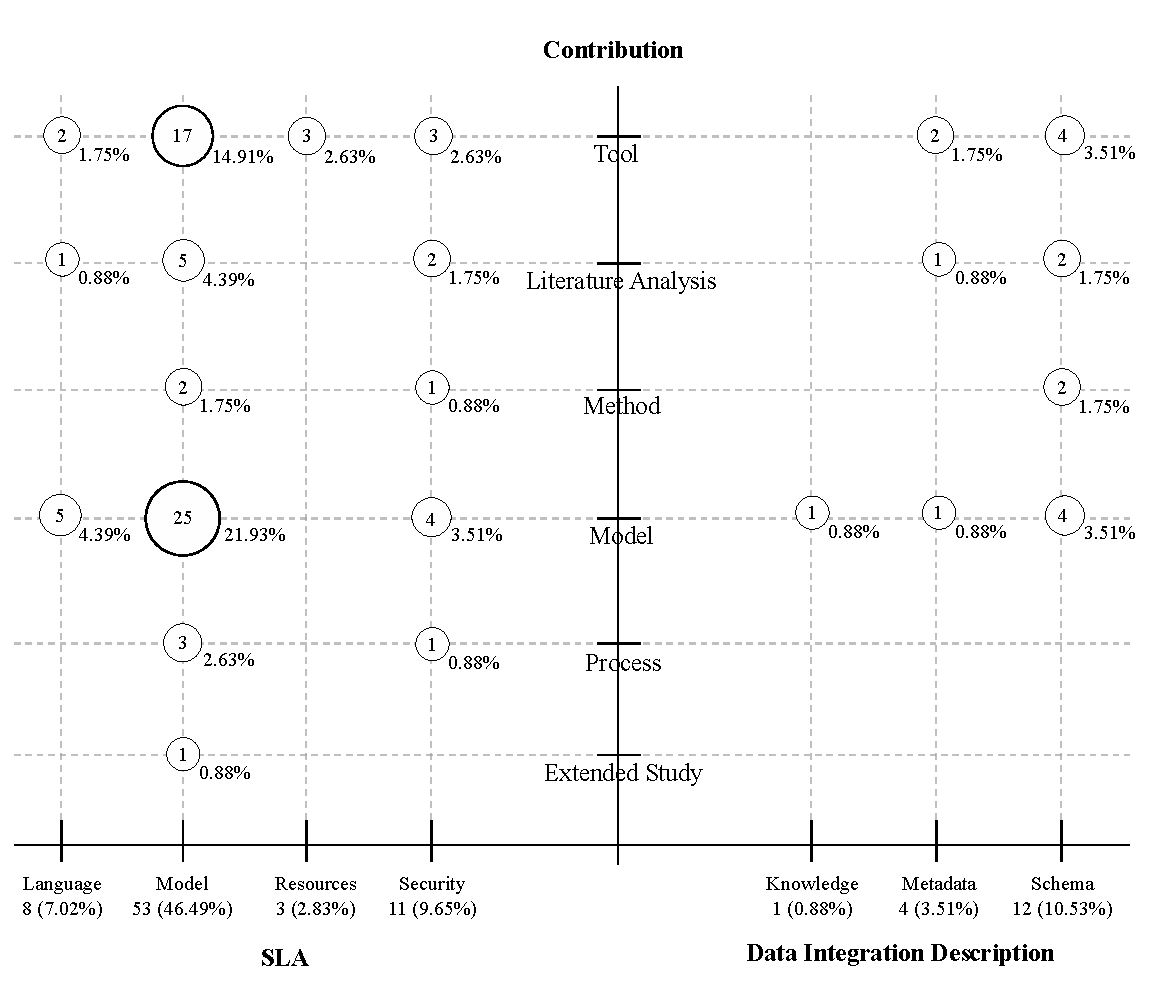
\includegraphics[scale=0.56]{figs/bubble-charts/Contribution-SLA-DIdescription.pdf} 
\caption{Contribution, SLA and Data Integration Description}\label{fig:facet1}
\end{figure}

Combining the facet contribution with the facets SLA and data integration description 
(Figure~\ref{fig:facet1}) it is possible to obtain two analysis: 
(i) how the SLA has been applied to scientific works and which are the type of contribution 
most proposed by the authors; and (ii) which are the most applied data integration description
strategy in papers and which are the most type of contribution associated to these works. 
Looking to the figure you can note that models for SLA have been the focus in the papers 
(53 appearances - 46.49\%) followed by Security (11 appearances - 9.65\%), Language 
(8 appearances - 7.02\%) and Resources (3 appearances - 22.83\%).
Analyzing the figure is also possible to observe that Model (34 appearances - 29.82\%) and 
Tool (25 appearances - 21.93\%) are the mainly type of contribution proposed in the papers 
followed by Literature Analysis (8 appearances - 7.02\%), Process (4 appearances - 3.51\%), 
Method (3 appearances - 2.63\%) and Extended Study (1 appearance - 0.88\%).
Regarding the data integration description, Schema (12 appearances - 10.53\%) is the most 
applied dimension followed by Metadata (4 appearances - 3.51\%) and Knowledge (1 appearance - 0.88\%).

\subsection{Combining the facets Data Integration Environment, Contribution and Research}

\begin{figure}[h]
\centering
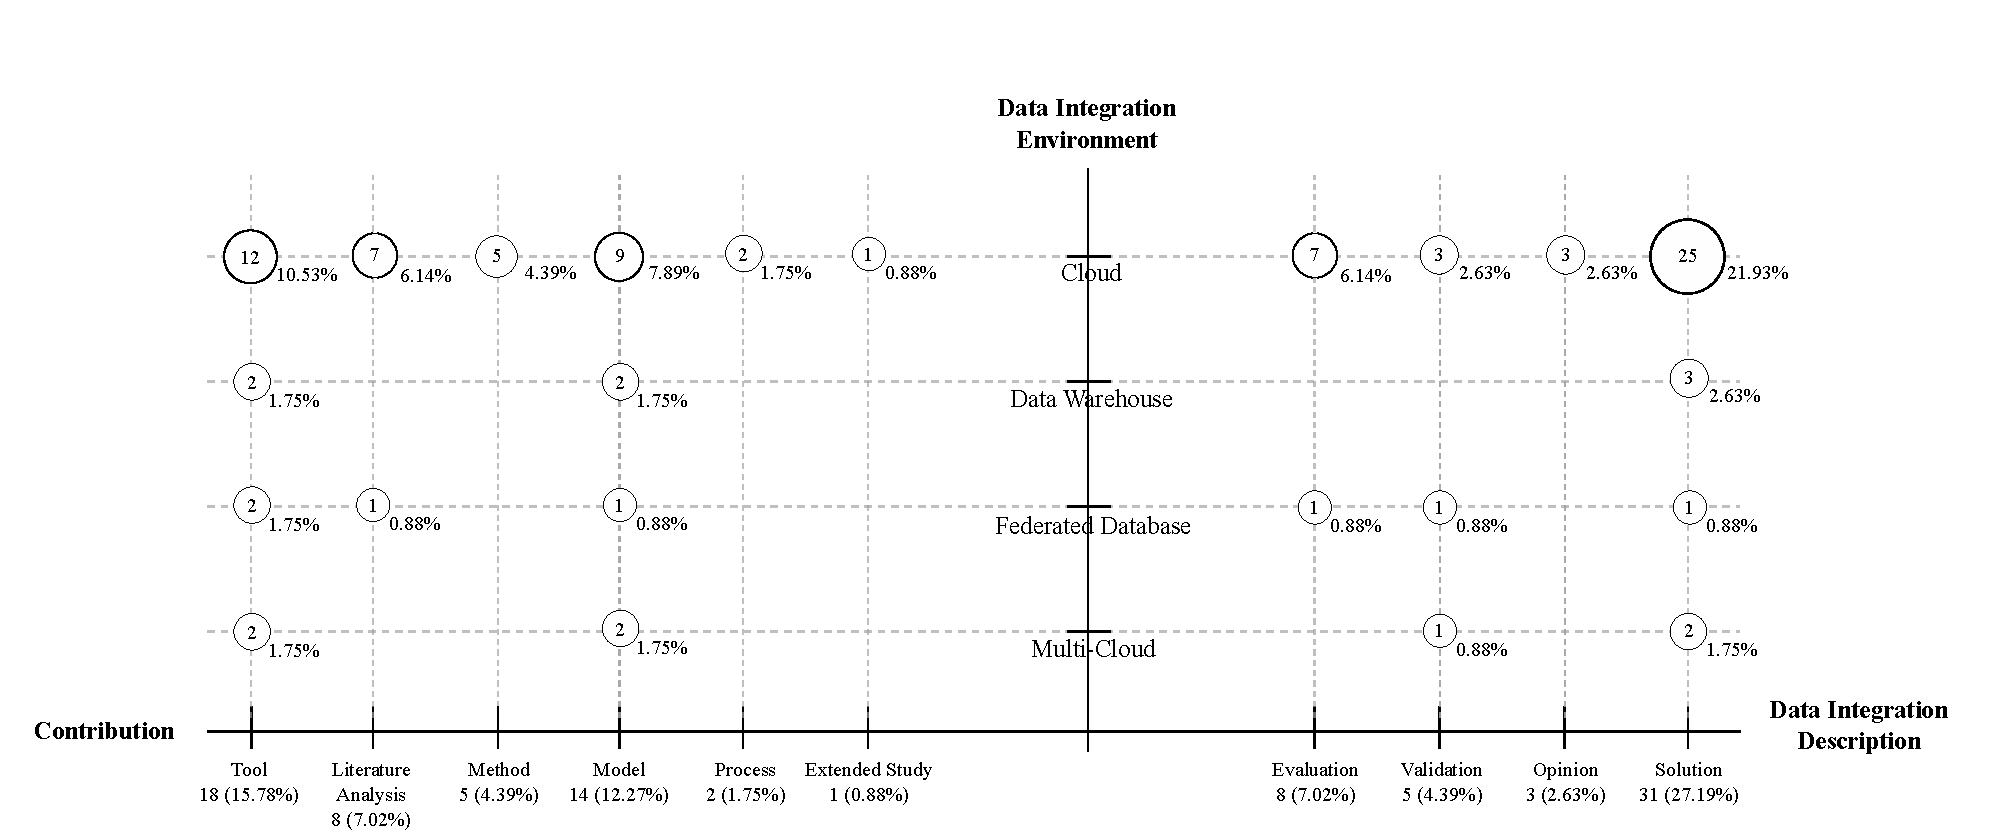
\includegraphics[scale=0.48]{figs/bubble-charts/DI-Environment-Contribution-Research.pdf}
\caption{facets Data Integration Environment, Contribution and Research}\label{fig:facet2}
\end{figure}

Combining the facet data integration environment with the facets contribution and research 
(Figure~\ref{fig:facet2}) it is possible to observe which are the most proposed type of
contribution and research applied to the different data integration environments.  
Looking to the figure it is possible to identify that Tool (18 appearances - 15.78\%) and 
Model (14 appearance - 12.27\%) are the mainly type of contribution developed, 
followed by Literature Analysis (8 appearances - 7.02\%), Method (5 appearances - 4.39\%) 
Process (2 appearances - 1.75\%) and Extended Study (1 appearance - 0.88\%).
Analyzing the figure is also possible to observe that Solution (31 appearances - 27.19\%) is 
the type of research most proposed, 
followed by Evaluation (8 appearances - 7.02\%), Validation (5 appearances - 4.39\%) and
Opinion (3 appearances - 2.63\%).

\iplacido{`Old' figure 3 deleted\ldots} 
 
% \subsection{Combining the facets SLA and Contribution}
% 
% Combining the facet SLA with the facet contribution (Figure~\ref{fig:facet3}) it is possible 
% to observe how the SLA has been applied to scientific works and which are the type of contribution 
% most proposed by the authors.
% Looking to the figure you can remark that models for SLA have been the focus of the most papers 
% (53 appearances).
% Analyzing the figure is also possible to observe that Model (34 appearances - 29.82\%) and 
% Tool (25 appearances - 21.93\%) are the mainly type of contribution proposed in the papers 
% followed by Literature Analysis (8 appearances - 7.02\%), Process (4 appearances - 3.51\%), 
% Method (3 appearances - 2.63\%) and Extended Study (1 appearance - 0.88\%).
% 
% \begin{figure}[h!]
% \centering
% 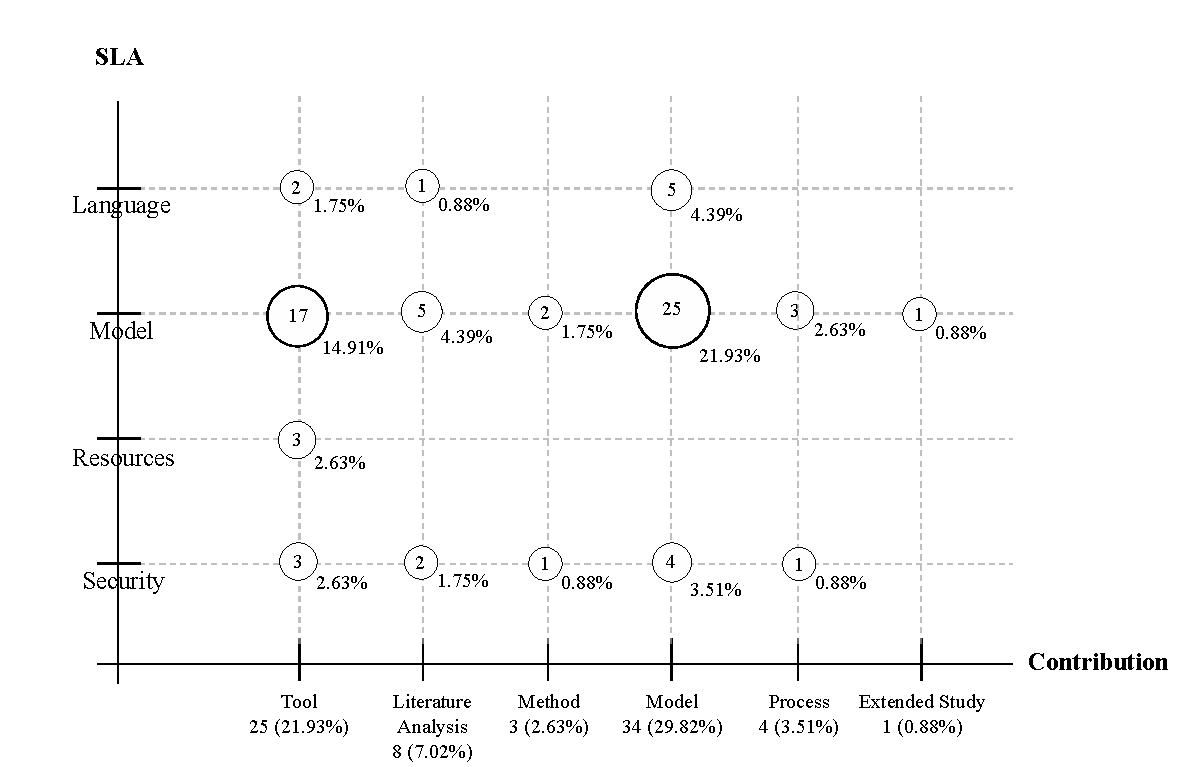
\includegraphics[scale=0.65]{figs/bubble-charts/SLA-Contribution.pdf}
% \caption{Facets SLA and Contribution}\label{fig:facet3}
% \end{figure}


\subsection{Combining the facets Data Quality, Data Integration Environment and Data Integration Description}

Combining the facet data quality with the facets data integration environment and data integration description
(Figure~\ref{fig:facet4}) it is possible to note which quality of service parameters have been applied most in
data integration studies.
It is also possible to identify which are the most applied data integration environment and description.
First of all, security and privacy are the most applied QoS parameter (5 appearance - 4.39\%)
followed by the other dimensions (1 appearance - 0.88\%). 
The figure also shows that SLA has not been widely used in order to address data integration solutions
(1 appearance) which reinforces our main objective of integrate SLA, data integration and multi-cloud 
environments. 
Analyzing the figure is also possible to observe that the most deployed data integration environment is 
the cloud (9.68\%) followed by multi-cloud (4.39\%), federated databases (1.75\%) and data warehouse (0.00\%).
The data integration description dimensions had the same percentage for schema, knowledge and metadata (2 appearance - 1.75\%)

\begin{figure}[!h]
\centering
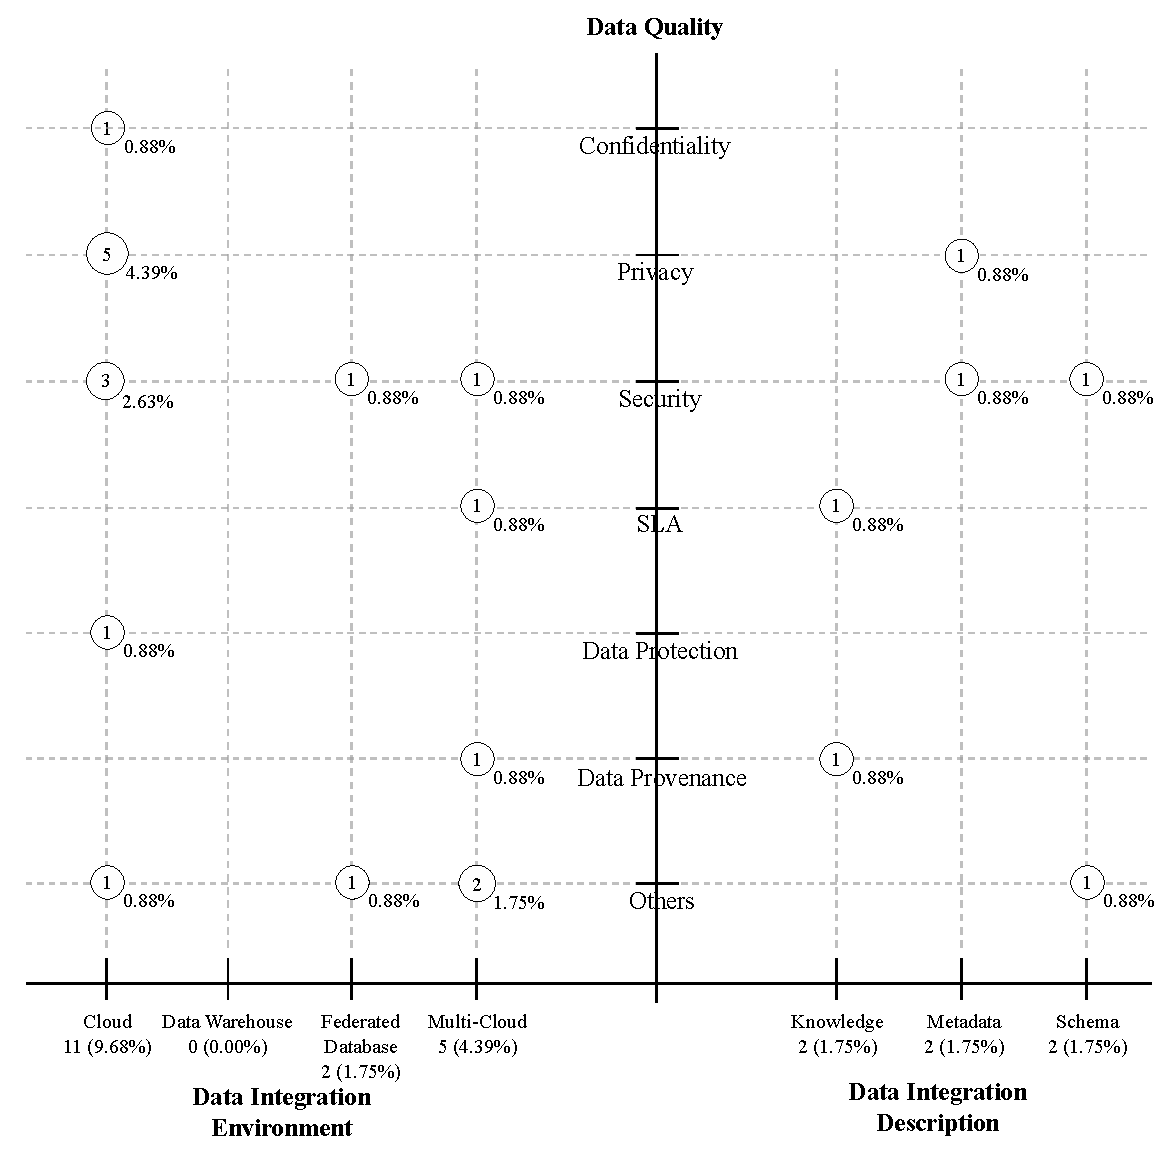
\includegraphics[scale=0.53]{figs/bubble-charts/Data-Quality-DI.pdf}
\caption{Facets Data Quality, Data Integration Environment and Data Integration Description}\label{fig:facet4}
\end{figure}

%-[END]-----------------------------------------------------------------------



%-[BEGIN]-----------------------------------------------------------------------
\section{Considering SLA and Data Integration on Multi-Cloud}
%-[END]-----------------------------------------------------------------------



%-[BEGIN]-----------------------------------------------------------------------
\section{Conclusion and final remarks}
 %-[END]-----------------------------------------------------------------------

%% References with bibTeX database:

\bibliographystyle{plain}
 \bibliography{bibliography,publications}


\end{document}

%%
%% End of file `elsarticle-template-1a-num.tex'.
